\documentclass[12,french]{report}
\usepackage{geometry}
\geometry{vmargin=3cm, hmargin=3cm}
\usepackage[T1]{fontenc}
\usepackage[utf8]{inputenc}
\usepackage[french]{babel}
\usepackage{graphicx}
\usepackage{amsmath}
\usepackage{amssymb}
\usepackage{sectsty}
\usepackage{authblk}
\usepackage{algpseudocode}
\usepackage{algorithm}
\usepackage{xspace}
\usepackage{mathtools}
\usepackage{mathrsfs}
\usepackage{enumitem}
\usepackage{titlesec}
\usepackage{hyperref}
\usepackage{xcolor}
\usepackage[justification=centering]{caption}
\usepackage{float}
\usepackage{tabto}

\usepackage{listings}
\usepackage{cleveref}

\renewcommand{\lstlistingname}{Code}
%\renewcommand{\figurename}{Fig.}

\lstdefinestyle{chstyle}{%
backgroundcolor=\color{gray!12},
basicstyle=\ttfamily\small,
showstringspaces=false,
numbers=left}

%\AddThinSpaceBeforeFootnotes
%\FrenchFootnotes

\titleformat{\chapter}[hang]{\bf\Huge}{\thechapter.}{2pc}{}
\titlespacing*{\chapter}{10pt}{0pt}{40pt}[0pt]
\newcommand{\HRule}{\rule{\linewidth}{0.5mm}}

\providecommand{\keywords}[1]{\textbf{\textit{Keywords:}} #1}
\bibliographystyle{apalike}

\usepackage{hyperref}

\begin{document}
\hypersetup{pdfborder=0 0 0}

\begin{titlepage}

\begin{center}
	\vspace*{\stretch{1}}	
	\textsc{{\LARGE Institut national des sciences appliquées de Rouen} \\ 			\vspace{6mm} {\Large INSA de Rouen}} \\
	\vspace{5mm}
	
\includegraphics[width=0.4\textwidth]{./Images/insa}\\[1.0 cm]

	\textsc{\Large Projet POOA GM4}\\[0.6cm]

	% Title
	\HRule \\[0.5cm]
	{ \Huge \bfseries Cahier de spécification - Tricount}\\[0.2cm]
	\HRule \\[0.75cm]

	
\includegraphics[width=0.7\textwidth]{./Images/Tricount}\\[0.9 cm]

	% Author and supervisor
	\begin{minipage}{0.4\textwidth}
		\begin{flushleft} \large
			\emph{Auteurs:}\\
			Thibaut \textsc{André-Gallis} \\
			{\small\href{mailto:thibaut.andregallis@insa-rouen.fr}{thibaut.andregallis@insa-rouen.fr}} \\
			Kévin \textsc{Gatel} \\
			{\small\href{mailto:kevin.gatel@insa-rouen.fr}{kevin.gatel@insa-rouen.fr}}\\
			Hugo \textsc{Merelle} \\
			{\small\href{mailto:hugo.merelle@insa-rouen.fr}{hugo.merelle@insa-rouen.fr}}\\
			Marion \textsc{Mesnil} \\
			{\small\href{mailto:marion.mesnil@insa-rouen.fr}{marion.mesnil@insa-rouen.fr}}\\
		\end{flushleft}
	\end{minipage}
	\begin{minipage}{0.4\textwidth}
		\begin{flushright} \large
			\emph{Enseignants:} \\
			Cecilia \textsc{Zanni-Merk} \\
			{\small\href{mailto:cecilia.zanni-merk@insa-rouen.fr}								{cecilia.zanni-merk@insa-rouen.fr}}\\
		\end{flushright}
	\end{minipage}
	\vspace*{\stretch{1}}

	\vfill
	{\large 6 décembre 2021}
\end{center}
\end{titlepage}

\tableofcontents
\listoffigures

\renewcommand{\chaptername}{}
\chapter*{Introduction}
\addcontentsline{toc}{chapter}{Introduction}

Tricount est une application qui permet d'organiser les dépenses de groupe. Ses utilisations sont multiples, elle permet notamment la répartition équitable des dépenses du groupe et le fait de pouvoir rembourser facilement quelqu'un si besoin. Elle peut également faire l’objet d’un récapitulatif de compte.\\

Dans ce projet on se propose de réaliser un Tricount à notre échelle, c'est -à -dire une application “locale” entre plusieurs clients (6 maximum) et un serveur. Le terme local est utilisé dans le sens où les clients peuvent se connecter au serveur s'ils partagent le même réseau.\\

L’utilisateur qui lance le serveur est appelé administrateur. Lui et lui seul a le droit d’ouvrir et/ou fermer l’application lorsqu’il le souhaite. Les autres utilisateurs ne peuvent se connecter à l’application que lorsque le serveur est ouvert au préalable par l’administrateur. \\

Lorsque le serveur est fermé toutes les données sont perdues. Nous ne stockons pas les données en local, tout se fait dans le serveur lorsqu’il est ouvert.\\

Dans un premier temps, nous allons voir différents diagrammes afin de clarifier la manière d’aborder le sujet. Puis dans un second temps, nous allons implémenter l’application en Java et commenter les éventuelles difficultées rencontrées.

\chapter{Diagrammes UML}

\section{Cas d'utilisation}

\begin{figure}[H]
	\center
	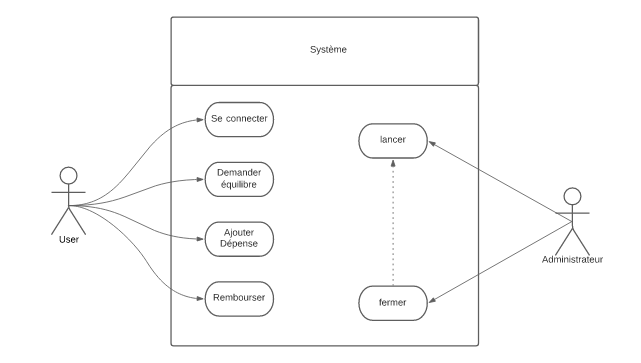
\includegraphics[width=0.7\textwidth]{./Images/Use-Case}
	\caption{Diagramme de cas d'utilisation}
\end{figure}\vspace{0.2cm}

Dans ce diagramme on distingue les deux cas suivants : l’administrateur et l’utilisateur de l’application. Le premier permet de lancer l’application puis de l'arrêter, alors que les “users” utilisent l’application suivant quatre options lorsque cette dernière est bien lancée.

\section{Séquence}

Le diagramme de séquence représentant l’option “Se connecter” pour l’utilisateur est représenté sur chacun des trois diagrammes de séquence suivants.\\

Le diagramme de séquence de l’option “Demander équilibre” est le suivant :\\

\begin{figure}[H]
	\center
	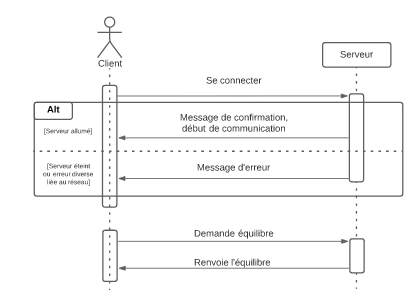
\includegraphics[width=0.7\textwidth]{./Images/Sequence_1}
	\caption{Diagramme de séquence "Demander Equilibre"}
\end{figure}\vspace{0.2cm}

Afin de pouvoir “Demander équilibre” au serveur, nous devons nous assurer que l’utilisateur est connecté au serveur. Dans le cas où l’utilisateur est bien connecté, un message de confirmation est envoyé à l’utilisateur et la requête peut commencer à être traitée, dans le cas contraire un message d’erreur est envoyé et la requête est renvoyée. Si l’utilisateur est correctement connecté au Serveur alors le Serveur envoie la liste des utilisateurs de l’application à l’utilisateur en les informant s’ils sont “en avance” ou “en retard” par rapport aux autres utilisateurs selon une somme d’argent indiquée.\\


Le diagramme de séquence de l’option “Ajouter dépense” est le suivant :\\

\begin{figure}[H]
	\center
	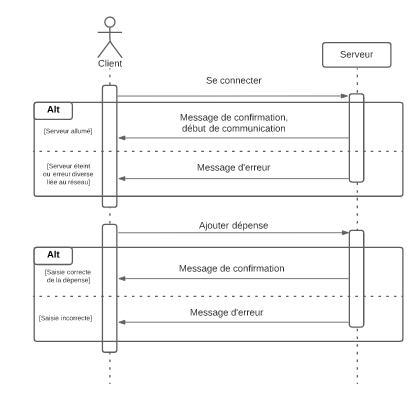
\includegraphics[width=0.7\textwidth]{./Images/Sequence_2}
	\caption{Diagramme de séquence "Ajouter dépense"}
\end{figure}\vspace{0.2cm}

Même chose que pour “Demander équilibre” l’utilisateur doit être connecté à l’application afin de pouvoir demander cette requête au Serveur. La dépense doit être positive et l’utilisateur doit au moins “cocher” une personne sur les 6 de manière à répartir la dépense équitablement. Le cas où l’utilisateur “coche” uniquement lui-même doit être rejeté. Un message de confirmation est envoyé à l’utilisateur si la requête s’est bien passée, un message d’erreur est retourné dans le cas contraire.\\

Le diagramme de séquence de l’option “Rembourser” est le suivant :\\

\begin{figure}[H]
	\center
	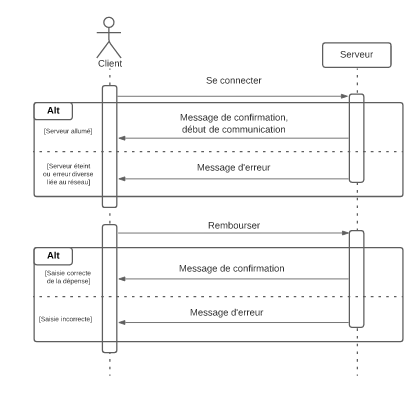
\includegraphics[width=0.7\textwidth]{./Images/Sequence_3}
	\caption{Diagramme de séquence "Rembourser"}
\end{figure}\vspace{0.2cm}

De la même manière que les précédents, l’utilisateur doit être connecté à l’application afin de pouvoir demander cette requête au Serveur. La somme du remboursement doit être également positive, et l’utilisateur doit “cocher” une et une seule personne (pas lui même) afin de le rembourser. Un message de confirmation est envoyé à l’utilisateur si la requête s’est bien déroulée, un message d’erreur est retourné dans le cas contraire.

\section{Modèle du domaine et diagramme de classe}

Nous avons réalisé le diagramme de modèle du domaine suivant :\\

\begin{figure}[H]
	\center
	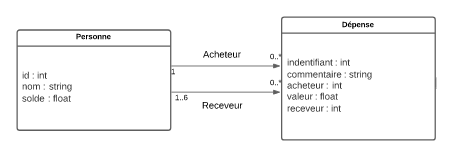
\includegraphics[width=0.7\textwidth]{./Images/Modele}
	\caption{Diagramme de modèle du domaine}
\end{figure}\vspace{0.2cm}

et le diagramme de classe suivant :\\

\begin{figure}[H]
	\center
	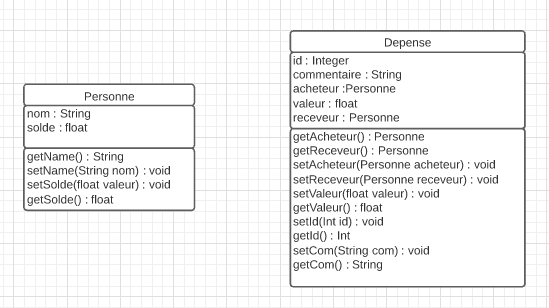
\includegraphics[width=0.7\textwidth]{./Images/Classe}
	\caption{Diagramme de classe}
\end{figure}\vspace{0.2cm}


Comme on peut le voir ci-dessus on peut distinguer 2 classes Personnes et Dépenses qui sont liées entre elles. Commençons d’abord par nous intéresser à chacune d’entre elles :\\

\begin{itemize}[label=\textbullet]
	\item \emph{Personne} :
La classe Personne représente un utilisateur de l’application tricount. Il va donc posséder deux variables d’instances, son nom qui sera une chaîne de caractères et son solde représenté par un flottant.
	\item \emph{Dépense} :
La classe dépense représente une dépense évidemment mais plus particulièrement une transaction entre deux personnes. Elle est définie par 5 variables : son identifiant qui sera un entier, un commentaire qui décrira à quoi correspond dans la vraie vie cette dépense (ex tickets de bus), une valeur flottante et puis un acheteur et un receveur qui seront des personnes.
\end{itemize}\vspace{0.5cm}


Ces deux classes sont liées car une dépense relie deux personnes l’une acheteuse et l’autre receveuse. S’il n’y a pas d’acheteur alors il ne peut y avoir de dépense. Chaque dépense est liée à uniquement un acheteur et un receveur. Cependant un acheteur peut avoir effectué plusieurs dépenses et un receveur en avoir reçu plusieurs également. 
Il est nécessaire de préciser que dans notre cas nous avons décidé de considérer le receveur comme une seule personne mais nous allons également traiter le cas où une dépense concerne plusieurs receveurs en générant plusieurs dépenses qui posséderont le même identifiant et qui auront une valeur divisée par le nombre de receveurs. Chacune reliera l’acheteur et un des receveurs. 

\section{Maquette de l'application}

\begin{figure}[H]
	\center
	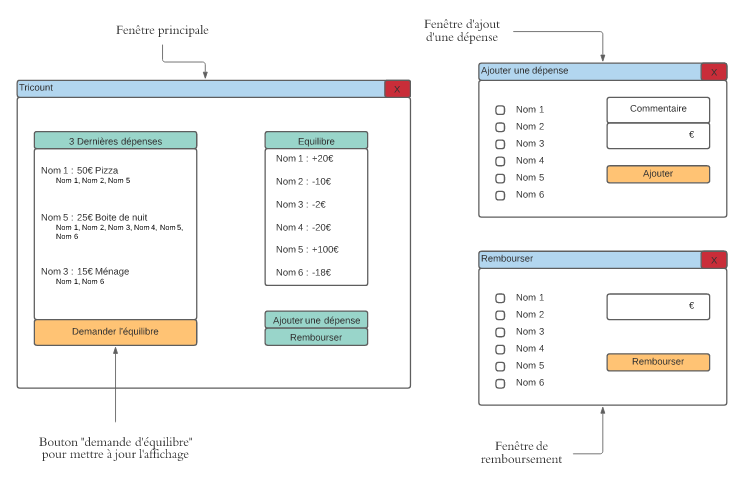
\includegraphics[width=0.7\textwidth]{./Images/Maquette}
	\caption{Maquette de l'application}
\end{figure}\vspace{0.2cm}

Elle peut être expliquée par le diagramme de navigation suivant.

\section{Navigation}

\begin{figure}[H]
	\center
	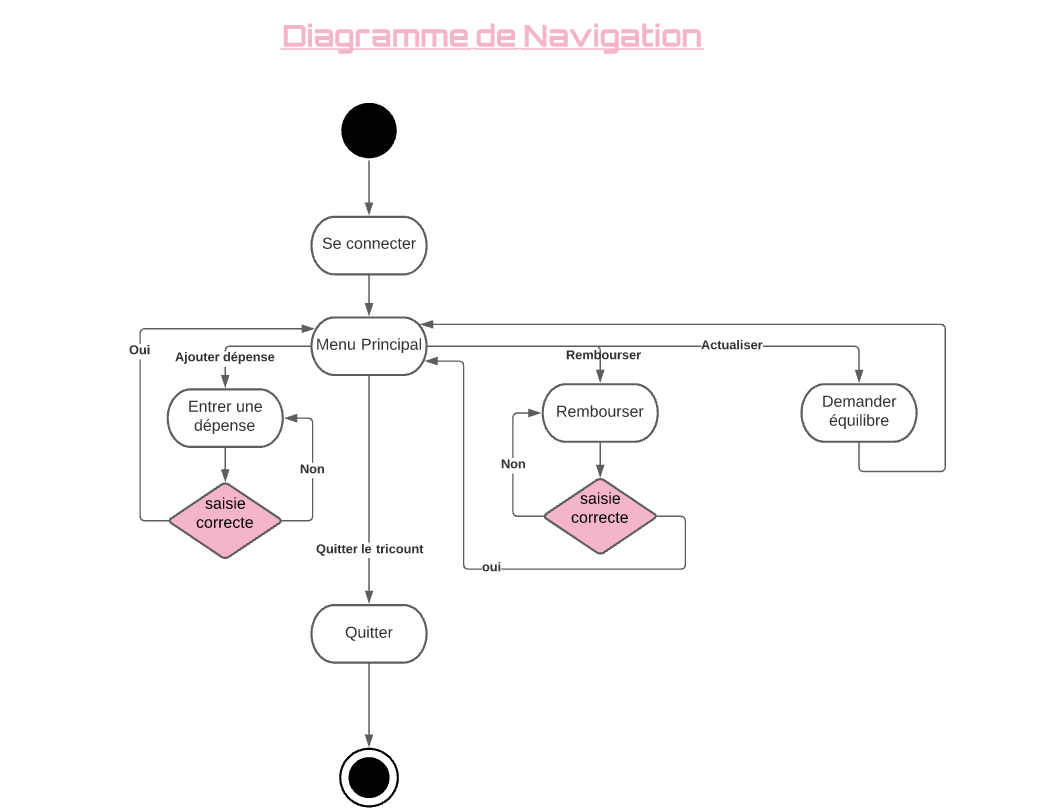
\includegraphics[width=0.7\textwidth]{./Images/Navigation}
	\caption{Diagramme de navigation}
\end{figure}\vspace{0.2cm}

L’utilisateur ouvre le tricount et se connecte, il arrive alors sur la fenêtre principale : le “menu principal”. Il peut donc entrer une dépense en cliquant sur le bouton “Ajouter une dépense”. Il arrive ensuite sur la fenêtre d’ajout d’une dépense et peut entrer le montant de sa dépense et sélectionner les personnes qui participent à cet achat (il peut se sélectionner lui-même si il paie également). Il clique ensuite sur “Ajouter”. Si sa saisie est correcte la dépense est prise en compte et il retourne sur la fenêtre principale, sinon un message d’erreur apparaît et il doit refaire sa saisie.
Le principe est le même pour le remboursement.
Ensuite, si l’utilisateur sélectionne le bouton “demander équilibre” l’affichage s’actualise avec les dernières dépenses.
Enfin, pour quitter le tricount il suffit de cliquer sur la croix rouge en haut à gauche de la fenêtre principale.\\

Les deux fonctions principales sont:\\

\begin{itemize}[label=\textbullet]
	\item \textit{public Int GetEquilibre(Personne Pers) throws RemoteException;}
Demande au serveur l’équilibre d’une personne. Elle la calcul à l’aide d’un tableau de dépense. Elle somme les achats et soustrait les dues.
	\item \textit{public void AddDepense(Int id, String Com, Personne acheteur, Int Val, Personne receveur) throws RemoteException;}
Elle permet d’ajouter une dépense et de rembourser ( en faisant une dépense inverse). Les dépenses sont stockées dans un tableau comme vu dans les premiers TDs. Une dépense à un client et un acheteur. Lorsque une dépense est crée elle sera automatiquement stockée plusieurs fois (le nombre de participant à la dépense).
\end{itemize}\vspace{0.5cm}

Pour notre Programme nous aurons deux utilisateurs :
L’administrateur qui lance et ferme le serveur.

Et les utilisateurs qui se connectent dans un premier temps. Puis ils ont 3 possibilitées:
Actualiser les soldes (l’équilibre de chaque personne).
Rembourser un autre utilisateur.
Ajouter une dépense.

Pour l’instant il y a peu de contraintes étant donné que nous sommes dans la phase de conception. Nous allons surement utiliser le RMI pour faire l'implémentation. 


\end{document}
